\chapter{Mapping} \label{chap:mapping}
    This chapter covers the development of the mapping system, starting with the process of projecting the depth image from the \ac{rgbd} camera into 3D space. After this, placing said 3D points into the heightmap buffer is covered. Finally, the \ac{gpu} implementation of the heightmap processing is described.
    \section{Overview}
        For accurate foot placement and localisation purposes, the robot makes use of two maps, a sparse map covering a large area, and a dense map covering a small area around the robot. The primary use of the sparse map is for localisation and extracting pose data, namely position, orientation, velocity, and angular rate, while the dense map is used to analyse the terrain and find an appropriate point to place the three swinging feet, which will become the supporting feet for the next half-cycle. While it is also possible to use the sparse map for autonomous path planning and navigation of the environment, this use case is outside the scope of this project.

        The localisation, sparse mapping, and pose estimation is performed by ORB-SLAM3 as described in \cite{campos2021orb}. The ORB-SLAM3 system was implemented on the hexapod robot by building UZ-SLAMLab's ORB-SLAM3 library, which can be found on github. A brief, user perspective overview of ORB-SLAM is given in section \ref{sec:orbslam3}.

        The dense mapping is performed by downsampling and projecting the \ac{rgbd} camera's depth image into 3D space, and using the pose acquired from ORB-SLAM3 to shift and rotate the projected points into the heightmap's reference frame. Once properly aligned to the map each projected point's z value is written into its corresponding heightmap cell.

    \section{Projecting the Depth Image to Map Space}
        In order to generate a heightmap from a \ac{rgbd} image, the 2D depth image must first be projected into the 3D camera reference frame. The 3D points in the camera reference frame can then be converted to 3D points in the heightmap reference frame using the pose estimate obtained from ORB-SLAM3. Finally, the 3D points in the heightmap reference frame are used to updated the 2.5D heightmap.

        The camera can be described by its intrinsic and extrinsic parameters. Extrinsic parameters characterise the cameras position in 3D space, and intrinsic parameters characterise the relationship between the image plane and 3D space, assuming that the camera reference frame is not displaced or rotated relative to the world reference frame \citep{hartley2003multiple}.

        Refer to figure \ref{fig:projection} as a visual aid regarding projection. Note that this figure is drawn from the perspective of projecting from the image plane into the world. If the objective was to project from the world onto the image plane, the projection center and image plane would swap places, causing the image to be inverted. Thus, this figure assumes that the image rotation has been corrected.
        \begin{figure}[h]
            \centering
            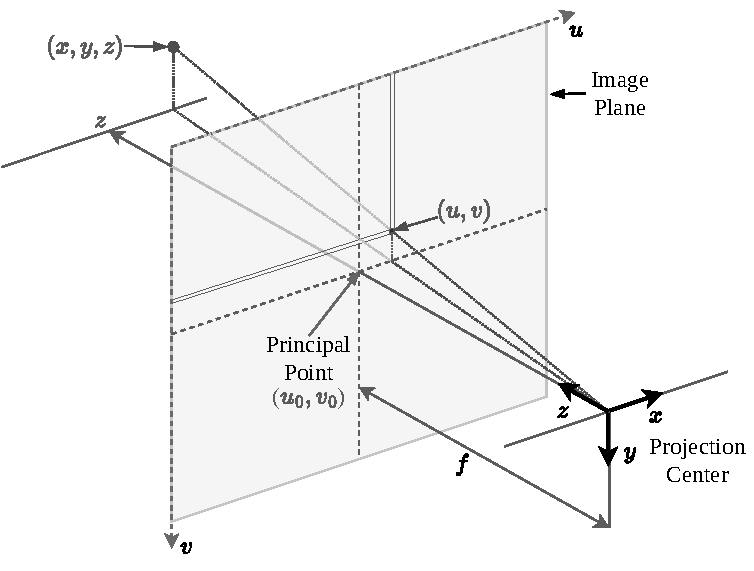
\includegraphics{Diagrams-Projection.drawio.pdf}
            \caption{Camera Projection}
            \label{fig:projection}
        \end{figure}

        \newpage
        \noindent
        Together the extrinsic and intrinsic matrices form the projection matrix, \(\bf{P}\), which is defined as
        \begin{equation} \label{eq:projection_matrix}
            \bm{P} = \bm{K}
            \begin{bmatrix}
                \bm{R} & \bm{T}
            \end{bmatrix}
        \end{equation}
        where \(\bm{K}\) is the intrinsic matrix and \(\begin{bmatrix} \bm{R} & \bm{T} \end{bmatrix}\) is the extrinsic matrix. \(\bf{R}\) and \(\bf{T}\) represent the rotation and translation relative to the world.
        The project matrix can be used to project a point in the 3D world space into the 2D image plane, as follows:

        \begin{equation} \label{eq:full_projection}
            \begin{bmatrix}
                u \\
                v \\
                1
            \end{bmatrix}
            = \bm{P}
            \begin{bmatrix}
                x \\
                y \\
                z \\
                1
            \end{bmatrix}
        \end{equation}
        where \(u,v\) are the pixel coordinates on the image plane and \(x,y,z\) are the coordinates in world space.

        The intrinsic matrix \(\bf{K}\) is defined as,
        \begin{equation} \label{eq:intrinsic}
            \bm{K} =
            \begin{bmatrix}
                \alpha_x & \gamma   & u_0 \\
                0        & \alpha_y & v_0 \\
                0        & 0        & 1
            \end{bmatrix}
        \end{equation}
        with the focal length represented by,
        \[\alpha_x = f \cdot m_y\]
        \[\alpha_y = f \cdot m_x\]
        where \(m_x\) and \(m_y\) are the inverse of the width and height of a image plane pixel, \(f\) is the focal length, and \((u_0,v_0)\) is the principal point, ideally located at the center of the image plane. The skew coefficient, \(\gamma\), is often, and in this case, 0.

        The extrinsic matrix is defined below
        \begin{equation}\label{eq:extrinsic}
            \begin{bmatrix}
                \bm{R} & \bm{T}
            \end{bmatrix}
            =
            \begin{bmatrix}
                \bm{R}_{3\times3} & \bm{T}_{3\times1} \\
                \bm{0}_{1\times3} & 1
            \end{bmatrix}
        \end{equation}
        where \(\bm{R}\) characterises the camera's rotation relative to the world frame and \(\bm{T}\) is the position of the world frame's origin expressed in the camera coordinate frame.

        For ease of preprocessing, the 2D points in the camera's image plane are first projected into the 3D camera coordinate frame. In other words, the extrinsic matrix is omitted from equation \ref{eq:full_projection}. The projection from the 3D camera frame onto the 2D image plane is therefore given by

        \begin{equation} \label{eq:local_projection}
            \begin{bmatrix}
                u \\
                v \\
                1 \\
                1/z
            \end{bmatrix}
            = \frac{1}{z}
            \begin{bmatrix}
                \alpha_x & 0 & u_0 & 0 \\
                0 & \alpha_y & v_0 & 0 \\
                0 & 0 & 1 & 0 \\
                0 & 0 & 0 & 1
            \end{bmatrix}
            \begin{bmatrix}
                x\\
                y\\
                z\\
                1
            \end{bmatrix}
        \end{equation}
        Rearranging this equation, the corresponding 3D point in the world frame can be calculated from the 2D point in the image plane, given that the depth value for the 2D point is also available from the RGB-D image, as follows:
        \begin{align}
            z &= I_{u,v} \label{eq:proj_z}\\[0.2cm]
            x &= \frac{z(u - u_0)}{\alpha_x}\label{eq:proj_x} \\
            y &= \frac{z(v - v_0)}{\alpha_y}\label{eq:proj_y}
        \end{align}
        where \(I_{u,v}\) is the depth image value at pixel coordinates \(u,v\). For later use the 3D position \(\bm{p} \inrefframe{C}\) in the camera frame is defined as
        \begin{equation}\label{eq:pcam}
            \bm{p}\inrefframe{C}=
            \begin{bmatrix}
                x &y &z
            \end{bmatrix}^T
        \end{equation}

        \noindent
        The 3D positions in the camera frame can be converted to the corresponding 3D positions in the map frame, as follows:
        \begin{align} \label{eq:camera_to_map}
            \begin{split}
                \bm{p}\inrefframe{\fworld} &= \transframe{\bm{x}\inrefframe{\fcamera}}{\fcamera}{\fworld}\\ 
                &= \bm{q}_{\fcamera\fworld} \cdot \bm{p}\inrefframe{\fcamera} \cdot \bm{q}_{\fcamera\fworld}{-1} + \bm{p}\inrefframe{\fworld}_{C0}
            \end{split}
        \end{align}

        \noindent
        where \(\boldsymbol{p}\inrefframe{\fmap}\) is the position in the world frame, \(\boldsymbol{q}_{\fcamera\fworld}\) is the quaternion rotation of the world frame relative to the camera frame, and \(\boldsymbol{p}\inrefframe{\fmap}_{C0}\) is the position of the camera frame's origin in the world frame.

    \newpage
    \section{Updating the Heightmap}
        Once the depth image is projected into map space, their x and y coordinates are used as indices to write their z value into the heightmap. The heightmap is stored in
        a 2D circular buffer, this means that as the robot moves around, old map data is erased to make room for new data. This structure is illustrated in figure \ref{fig:memory}.
        \begin{figure}[h]
            \centering
            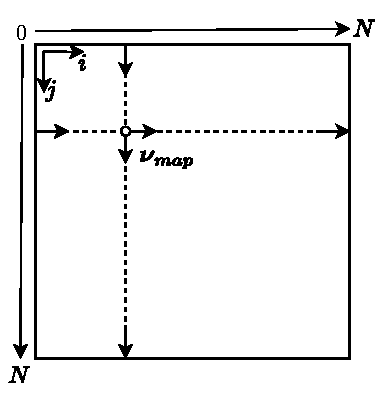
\includegraphics{Diagrams-Memory.drawio.pdf}
            \caption{2D Circular Buffer that stores Heightmap}
            \label{fig:memory}
        \end{figure}

        \noindent
        The heightmap buffer, \(\bm{M}\), is of size \(N \times N\) and is indexed by \([i,j]\). \(\boldsymbol{p}\inrefframe{\fmap}_r\) represents the robot's current position in the heightmap, note how this position wraps around when reaching the bounds of the buffer. The indices i and j are calculated as follows:
        \begin{align} \label{eq:map_index}
            \begin{split}
                i &= \lfloor x\inrefframe{\fworld} \Delta \rfloor \mod{N} \\
                j &= \lfloor y\inrefframe{\fworld} \Delta \rfloor \mod{N}
            \end{split}
        \end{align}
        where \([x\inrefframe{\fworld}, y\inrefframe{\fworld}]\) are the horizontal coordinates in the world frame, \(\Delta\) is the horizontal resolution of the heightmap, and \(N\) is the side length of the 2D array that stores the heightmap.
        
    \newpage
    \section{GPU Compute Pipeline}
        As the heightmap generation and heightmap scoring systems are essentially image manipulation processes, parallelisation of the algorithms is a very efficient way to increase computational speeds. Therefore, these algorithms are run in parallel on the Jetson nano's \ac{gpu} using OpenGLcompute shaders. This section describes the compute pipeline used to build and score the heightmap. The compute pipeline can be seen in figure \ref{fig:compute_pipe}.
        \captionsetup[figure]{oneside,margin={0cm,0cm}}
        \begin{figure}[h]
            \centering
            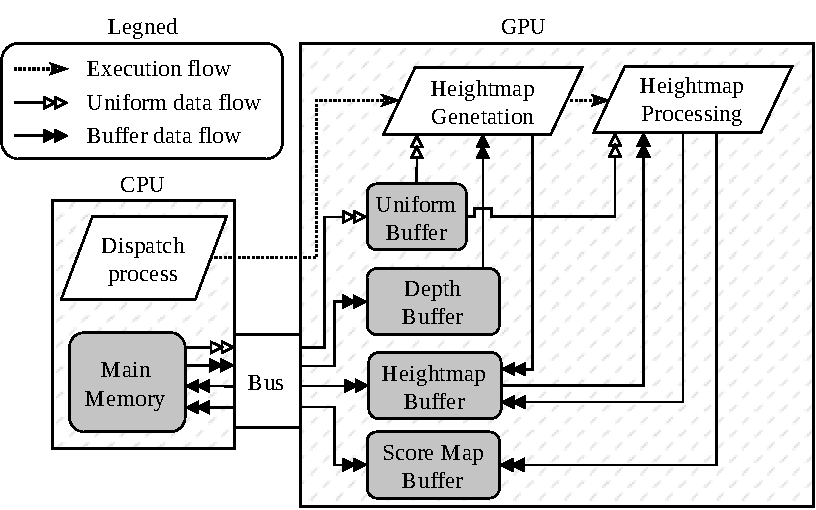
\includegraphics{Diagrams-ComputePipeline.drawio.pdf}
            \caption{Compute pipeline.}
            \label{fig:compute_pipe}
        \end{figure}
    
        \noindent
        As seen from figure \ref{fig:compute_pipe}, the \ac{gpu} pipeline is relatively simple, being comprised of only two stages, the heightmap generation stage and the heightmap processing stage. The heightmap generation stage executes for each pixel on the depth image, constructing the heightmap as described in the previous section.
        
        After the heightmap has been generated, the heightmap processing stage operates over the heightmap buffer. This stage has two tasks, to erase the old height data as the robot walks around, and to generate the score map, which will be described in chapter \ref{chap:optimisation}.
        
        \newpage
        \subsection{A note on GPU architecture}
            A process on a \ac{gpu} operates fully in parallel and the \ac{gpu} is highly optimised for parallelisation. Thus, there is a very specific execution structure that a \ac{gpu} process must abide by to perform at maximum efficiency, or to even function at all. This execution structure is as follows: As per \cite{nvidia_doc}, when writing compute code, a 3D size is specified, namely the localgroup size, \(\bm{N}_{l} = [X_l,Y_{l},Z_{l}]\). Next when the \ac{cpu} dispatchesa compute task, the workgroup count, is fed as parameter, \(\bm{n}_{w} = [x_{w},y_{w},z_{w}]\). The \ac{gpu} then initialises \(\bm{n}_w\) workgroups, and each workgroup initialises \(\bm{N}_l\) threads. These threads are executed into warps, or waves, which, depending on the architectures processor count,can be either 32 or 64 threads. To ensure maximum efficiency it is important that \(\bm{N}_l\) is divisible by the warp size.
            Originally, Nvidia \ac{gpu}s utilised a warp size of 32 and AMD GPUs a warp size of 64, however with AMD's latest RDNA architecture, the warp size could be either 32 or 64. For the mapping system developed in this project, a warp size of 32 was used.
            
            For the heightmap generation stage, a localgroup size of \(\bm{N}_{l} = [32,32,0]\) was used for a total of 1024 threads per workgroup, or in other words, 32 warps per workgroup.
            As for the heightmap processing stage, a localgroup size of \(\bm{N}_{l} = [32,32,32]\) was used, meaning 32768 threads, or 1024 warps per workgroup. As such, it is important that the camera images, the heightmap, and the score map are of a size divisible by 32.
            % A basic diagram of this execution scheme can be seen in figure \ref{fig:gpu_scheme}.
            % \begin{figure}[h]
            %     \centering
            %     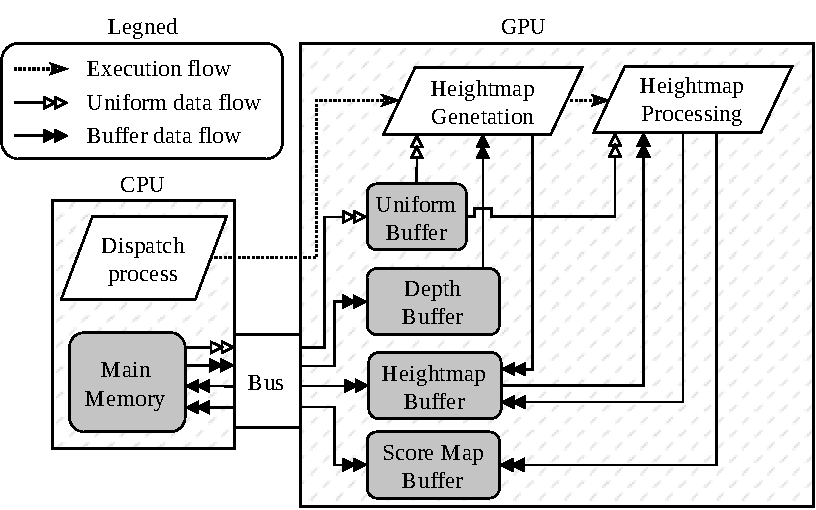
\includegraphics{Diagrams-ComputePipeline.drawio.pdf}
            %     \caption{GPU execution scheme.}
            %     \label{fig:gpu_scheme}
            % \end{figure}
        
            % \noindent
            While threads can directly communicate with each other within the same workgroup, direct communication across workgroups is impossible. If cross workgroup communication is desired, this must be performed using \ac{gpu} buffers, which are slower to access. Therefore, the processes were designed to operate fully independently from each other. Of course, data transfer between the \ac{cpu} and the \ac{gpu} is orders of magnitudes slower than accessing local buffers. For this reason, all communication between the \ac{cpu} and \ac{gpu} is kept to a minimum.
            
            Finally, it should be noted that, while it is possible to vary \(\bm{n_w}\) with each execution cycle, \(\bm{N_l}\) is a constant specified at compile time,
            and as such the number of threads per workgroup cannot be altered during operation.

    \newpage
    \section{Simultaneous Localisation and (Sparse) Mapping} \label{sec:orbslam3}
    This section provides a brief overview of the implementation and usage of ORB-SLAM3 from a user perspective.
    
    ORB-SALM3 operates by detecting features in the image streams coming from the connected camera. These features are then used to build a sparse feature map of the environment, subsequent features are used to expand the map. When trying to determine the camera's pose, the current image frame(s) of the camera is compared against the generated feature map, if the features detected in the current images are successfully matched to that in the map, the pose, relative to the feature map's origin, is returned as the robot's (or any other use case) current pose estimate.

    In this project ORB-SLAM3 is executed as a separate \ac{ros} node. This isolates ORB-SLAM3 from the rest of the system maximising modularity. The \ac{ros} node is subscribed to the color and depth streams originating from the \ac{rgbd} camera. The color and depth streams are used as inputs to the tracking function, which performs localisation. The tracking function then outputs the pose estimate, which is immediately published, with the same timestamp as the depth image attached. This is to ensure that the pose estimate and depth image used in generating the dense-map are synchronised.

    \newpage
    \section{Hardware Mapping Test}\label{sec:hardware_hmap}
        The mapping system described above was tested on the physical robot. This mapping test aimed to show how the physical hexapod maps various objects while in motion. The test consisted of the robot walking past various obstacles, while simultaneously generating a heightmap.

        Figure \ref{fig:hardware_map_diag} shows a top-down diagram of the placed obstacles used in this test, with the path the robot walks.
        \begin{figure}[h]
            \centering
            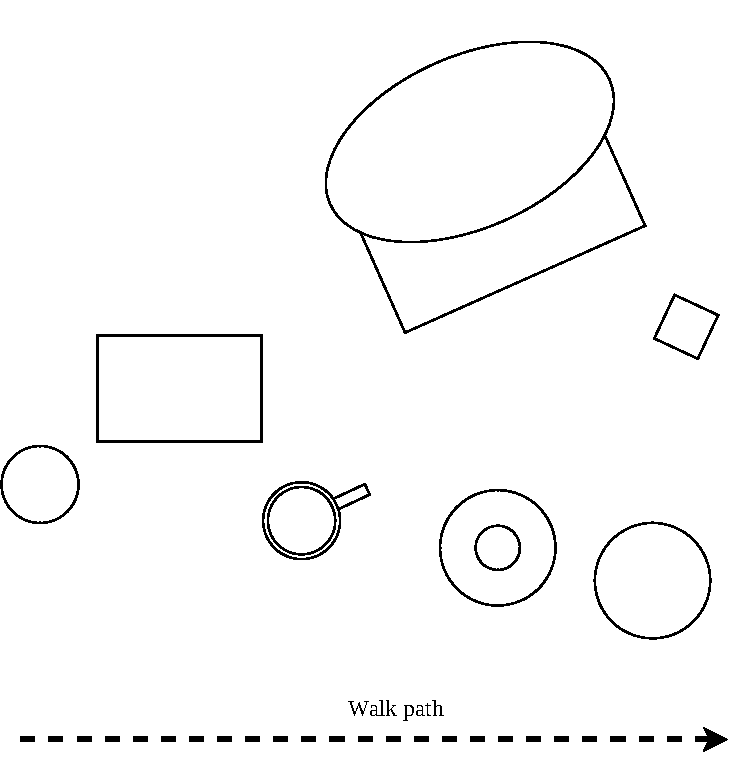
\includegraphics[clip, trim=0 0 0 0.5cm]{Diagrams-HardwareTest.drawio.pdf}
            \caption{Top-down diagram of the test setup.}
            \label{fig:hardware_map_diag}
        \end{figure}

        \noindent
        The test objects were selected to show a variety of obstacle types, with a variety of heights, that the robot might encounter, including sloped objects, spherical objects, objects with holes, and irregular objects.

        Figures \ref{fig:hardware_hmap_start}, \ref{fig:hardware_hmap_mid} and \ref{fig:hardware_hmap} show the heightmap, and its corresponding color frame, at the start middle and end of the
        robot's walking path. Please see \hyperlink{}{this video} of the test from the robot's perspective.
        
        \newpage
        \noindent
        Figure \ref{fig:hardware_hmap_start} shows the heightmap at the start of the generation, at this point the heightmap is essentially a direct representation of what is currently seen by the camera. This is quite clear by the shadows cast by both the robot's leg (on the left) and by the obstacles (the piggybank and box). In this static case
        very little noise is also present.
        \begin{figure}[h]
            \centering
            \hspace{-0.8cm}
            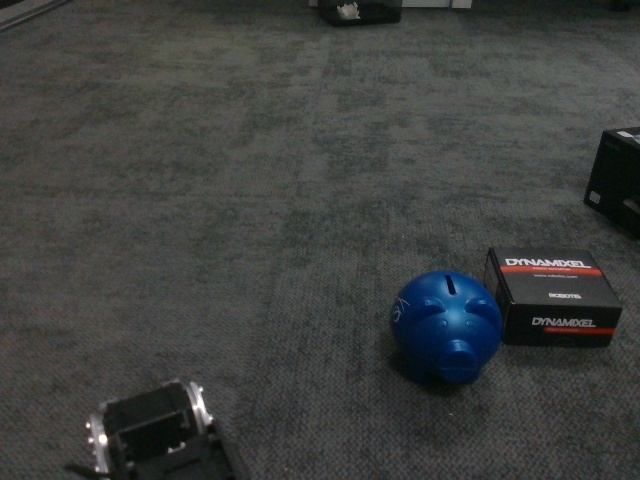
\includegraphics[width=.6\textwidth]{color_start.jpeg}
            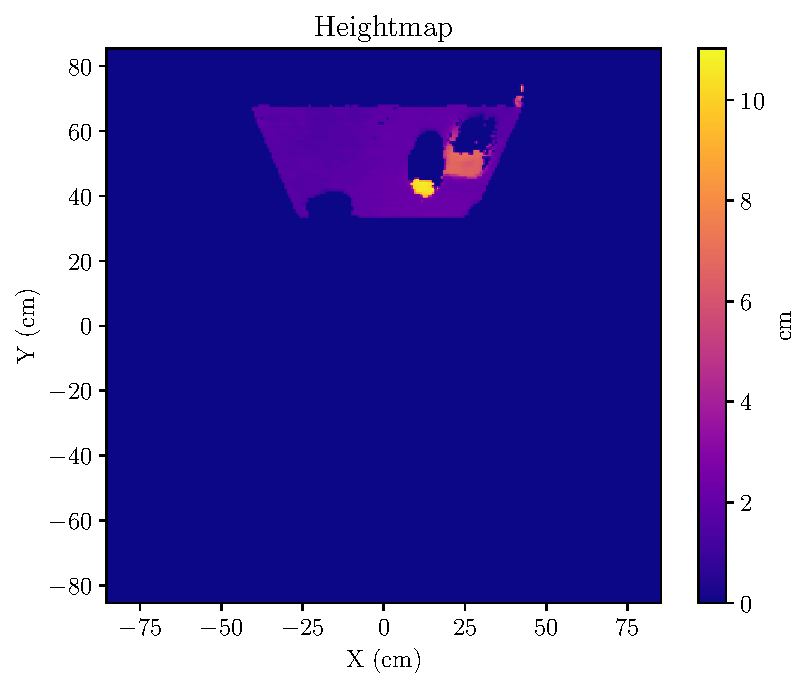
\includegraphics[width=.9\textwidth]{hmap_start.pdf}
            \caption{Colour frame at the start of walking path (Top). Heightmap generated at the start of the walking path (Bottom).}
            \label{fig:hardware_hmap_start}
        \end{figure}
        
        \newpage
        \noindent
        Figure \ref{fig:hardware_hmap_mid} shows the heightmap at a middle point of the path, here it can be seen how some of the shadows have been
        filled in by the movement of the camera. Particularly, the shadow caused by the robot leg is no longer present, and the shadows cast by the
        obstacles are reduced. The somewhat spherical pig object now also appears larger as part of the other side became visible.
        \begin{figure}[h]
            \centering
            \hspace{-0.8cm}
            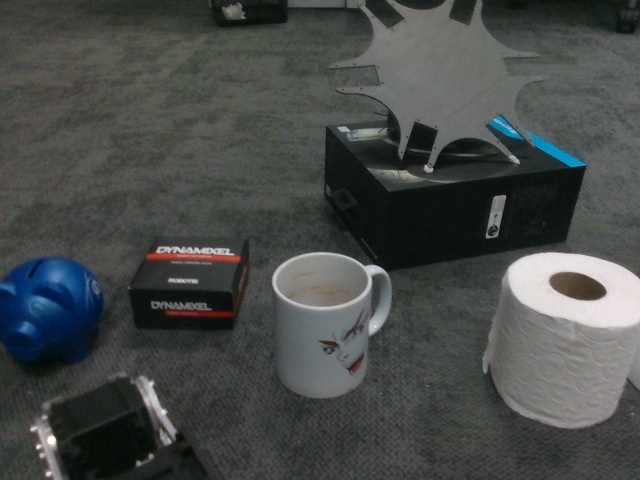
\includegraphics[width=.6\textwidth]{color_half.jpeg}
            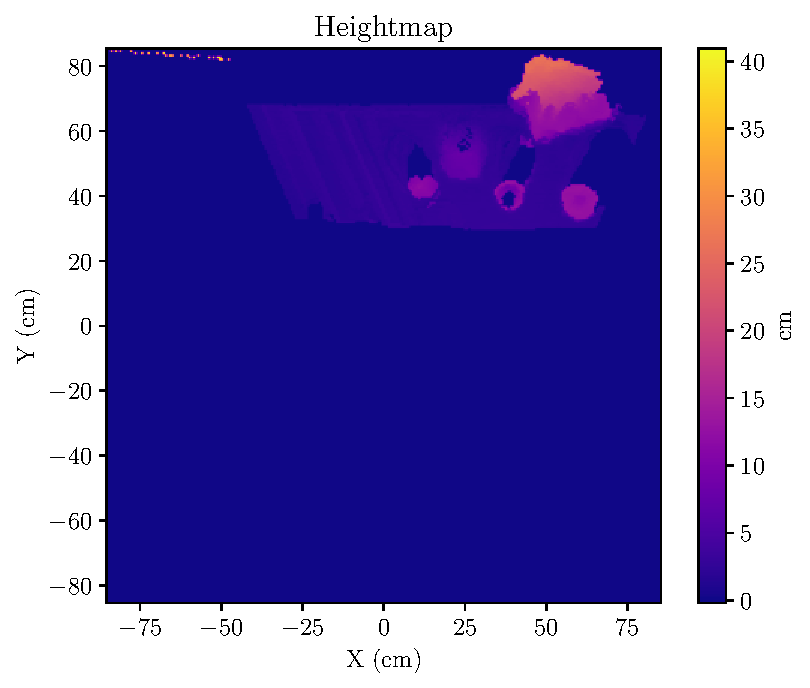
\includegraphics[width=.9\textwidth]{hmap_half.pdf}
            \caption{Colour frame at the middle of walking path (Top). Heightmap generated at the middle of the walking path (Bottom).}
            \label{fig:hardware_hmap_mid}
        \end{figure}

        \noindent
        In this heightmap however, noise is more prevalent, this is particularly visible when looking at the floor height, where distinct lines can be observed.
        These lines are the edge of the field of vision of the camera which is being moved to the right, and is caused by inaccuracies in the position estimation.

        \begin{figure}[h]
            \centering
            \hspace{-0.8cm}
            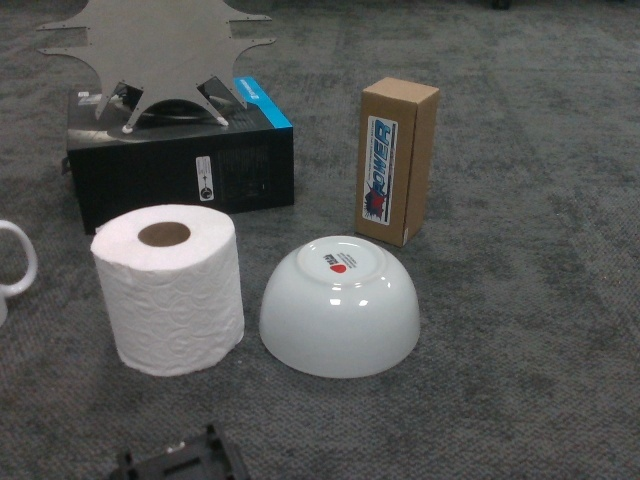
\includegraphics[width=.6\textwidth]{color.jpeg}
            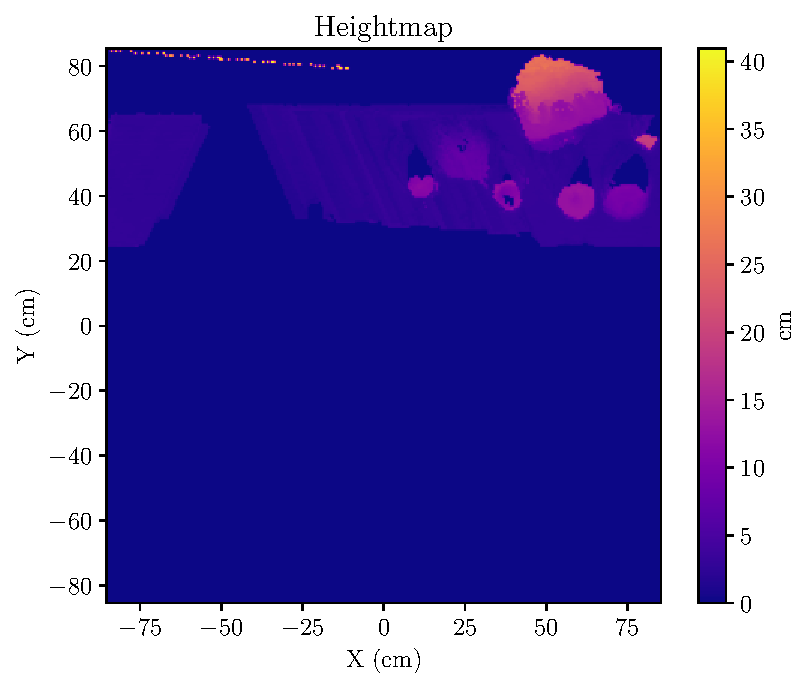
\includegraphics[width=.9\textwidth]{hmap.pdf}
            \caption{Colour frame at the end of walking path (Top). Heightmap generated at the end of the walking path (Bottom).}
            \label{fig:hardware_hmap}
        \end{figure}

        \noindent
        Finally, the heightmap generated at the end of the walking path can be seen in figure \ref{fig:hardware_hmap}. In this heightmap the shadows cast have been shrunk even more, and some additional objects became visible. The original objects are also now out of vision, but they persist on the heightmap. 

        Figure \ref{fig:hardware_pos}  show the pose estimate provide by the ORB-SLAM3 system during the hardware test, with each dot being an estimate. The blue dot indicates the start of the test and the red dot indicates the end of the test.
        \begin{figure}[h]
            \centering
            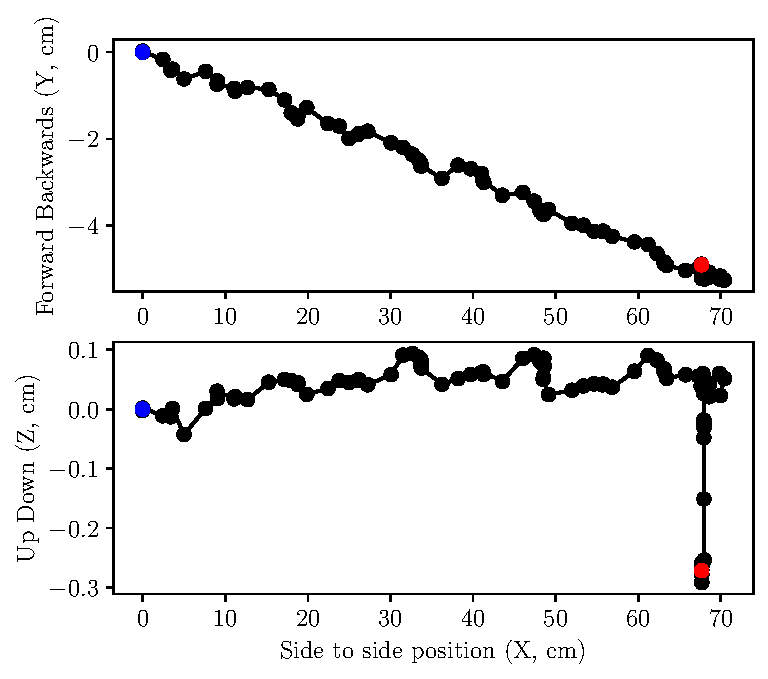
\includegraphics{pos.pdf}
            \caption{Pose estimate output from ORB-SLAM3}
            \label{fig:hardware_pos}
        \end{figure}

        \noindent
        As can be seen, the frequency of pose estimates causes there to sometimes be large jumps between estimates. This is especially noticeable at the end where the robot quickly lowers itself. If the system was further optimised to increase the frequency and consistency of estimates, the accuracy of the heightmap would also increase.

        % \noindent
        % Note that the line of motion is not aligned perfectly with the x-axis as stated in the test diagram in figure \ref{fig:hardware_map_diag}, this is due to slight user error while inputting the target velocity, but does not have any negative effects on the resultant heightmap.
    % \bigskip
    % \bigskip
    % \hrule
    % \smallbreak
    % \hrule
